% Copyright 2021 Edoardo Riggio

% Licensed under the Apache License, Version 2.0 (the "License");
% you may not use this file except in compliance with the License.
% You may obtain a copy of the License at

% 	http://www.apache.org/licenses/LICENSE-2.0

% Unless required by applicable law or agreed to in writing, software
% distributed under the License is distributed on an "AS IS" BASIS,
% WITHOUT WARRANTIES OR CONDITIONS OF ANY KIND, either express or implied.
% See the License for the specific language governing permissions and
% limitations under the License.

\documentclass{article}

\usepackage{hyperref, amsmath, graphicx, amssymb}
\usepackage{fancyvrb, newverbs, xcolor, tikz}

\usetikzlibrary{positioning}

\graphicspath{{./assets/}}
\definecolor{cverbbg}{gray}{0.93}

\newenvironment{cverbatim}
 {\SaveVerbatim{cverb}}
 {\endSaveVerbatim
  \flushleft\fboxrule=0pt\fboxsep=.5em
  \colorbox{cverbbg}{\BUseVerbatim{cverb}}%
  \endflushleft
}

\newenvironment{lcverbatim}
 {\SaveVerbatim{cverb}}
 {\endSaveVerbatim
  \flushleft\fboxrule=0pt\fboxsep=.5em
  \colorbox{cverbbg}{%
    \makebox[\dimexpr\linewidth-2\fboxsep][l]{\BUseVerbatim{cverb}}%
  }
  \endflushleft
}

\begin{document}
\begin{titlepage}
    \begin{center}
        \vspace*{1cm}
        
        \Huge
        \textbf{Theory of Computation Cheatsheet}
        
        \vspace{0.5cm}
        \LARGE
        
        \vspace{.5cm}
        
        Edoardo Riggio
   		  \vspace{1.5cm}
       
        \vfill
        
        \today
        
        \vspace{.8cm}
          \Large
          Theory of Computation - S.P. 2022 \\
        Computer Science\\
        Universit\`{a} della Svizzera Italiana, Lugano\\
        
    \end{center}
\end{titlepage}

\tableofcontents

\newpage

\section{Introduction}
The Turing Machine was invented by \textbf{Alan Turing} in 1936. A Turing Machine is a much more accurate model of a general-purpose computer than a PDA or FA. This type of machine can do anything that a real computer can. \\ \\
The following are some characteristics of a Turing Machine:

\begin{itemize}
	\item The input tape of the TM is infinite
	\item The input head of the TM can both read from and write to the tape
	\item The input head of the TM can move both left and right
	\item The RM has both accepting and rejecting states. Once it reaches such states, it accepts/rejects immediately -- i.e., it does not need to get to the end of the input.
\end{itemize}

\subsection{Formal Definition}
A Turing Machine is defined as follows:
\[ TM: (Q, \Sigma, G, \delta, q_0, q_{accept}, q_{reject}) \]
Where $Q$ is a \textbf{set of states}, $\Sigma$ is the \textbf{input alphabet}, $G$ is the \textbf{tape alphabet} -- where $\Sigma \subset G$, $\delta$ is the \textbf{transition function}, $q_0$ is the \textbf{initial state}, $q_{accept}$ is the \textbf{set of accepting states}, and $q_{reject}$ is the \textbf{set of rejecting states}.

\subsection{Configurations}
\subsubsection{Starting Configuration}
The starting configuration of $M$ on $\omega$ is $q_0 \omega$, which indicates that the machine is in the start stating state $q_0$. Moreover, the head of the TM is in the leftmost position.

\subsubsection{Accepting and Rejecting Configurations}
The accepting and rejecting configurations are the halting configurations. They do not yield any further configuration.

\subsection{Acceptance}
A Turing Machine is said to accept an input string $\omega$ if a sequence of configurations $C_1, C_2, \dots C_k$ exists where:

\begin{itemize}
	\item $C_1$ is the starting configuration
	\item $C_i$ yields $C_{i+1}$
	\item $C_k$ is the accepting configuration
\end{itemize}

\subsection{Turing-Recognizable Language}
A string collection is a TM's language if the TM \textbf{accepts} it. A TM is said to \textbf{recognize} a language if it accepts all and only those strings in the language. \\ \\
A language is said to be \textbf{Turing-recognizable} if some TM recognizes it. This means that a TM can accept, reject or loop.

\subsection{Turing-Decidable Language}
While the possible outcomes of a TM are \textit{accept}, \textit{reject} and \textit{loop}, a TM \textbf{decides} a language if it accepts all strings in the language, and reject all strings not in the language -- i.e., it never loops.

\subsection{Turing Machine Variants}
\subsubsection{Multitape Turing Machines}
This is a TM that has $k$ number of tapes. The transition function for this Turing Machine allows for reading, writing, and moving the heads on some or all tapes simultaneously. \\ \\
Every multitape Turing Machine has an equivalent single-tape Turing Machine.

\subsubsection{Non-Deterministic Turing Machines}
The machine may proceed according to several choices at any point in the computation. The resulting computation is a tree whose branches correspond to the various possibilities of the machine. \\ \\
A non-deterministic Turing Machine \textbf{accepts} if some branch of the computation leads to an accepting state. \\ \\
Every nondeterministic Turing Machine has an equivalent deterministic Turing Machine.

\section{Computability Theory}
We study unsolvability because knowing a problem cannot be solved helps us restate or simplify the problem.

\subsection{Solvability}
A problem is said to be solvable if we can find a Turing Machine that \textbf{decides} that problem.

\begin{center}
	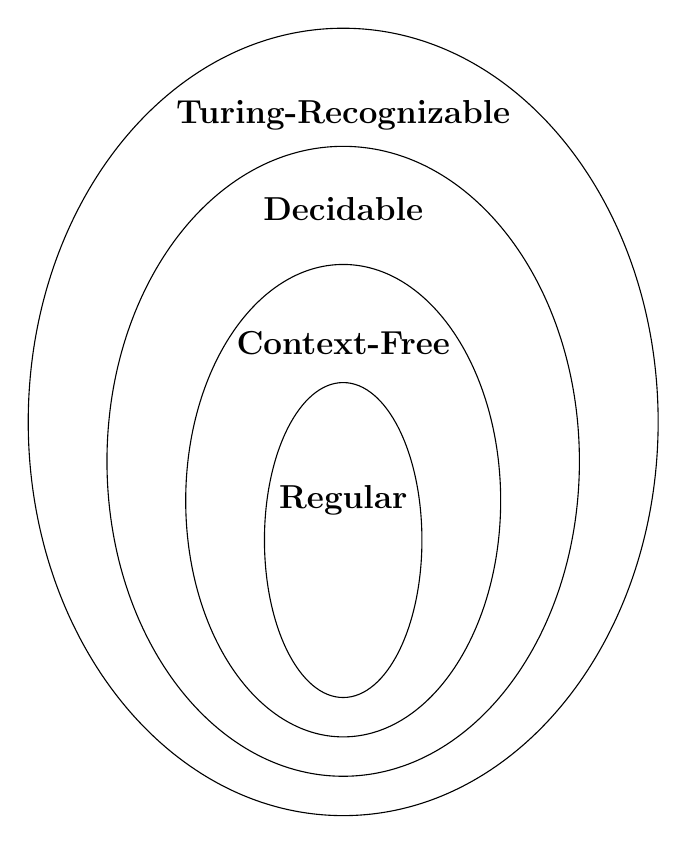
\begin{tikzpicture}
    	\begin{scope}
          \draw[draw = black] (0,0) ellipse (4 and 5);
      	  \draw[draw = black] (0,-0.5) ellipse (3 and 4);
       	  \draw[draw = black] (0,-1) ellipse (2 and 3);
      	  \draw[draw = black] (0,-1.5) ellipse (1 and 2);
    		\node at (0,3.9) (A) {\large\textbf{Turing-Recognizable}};
    		\node at (0,2.7) (B) {\large\textbf{Decidable}};
    		\node at (0,1) (C) {\large\textbf{Context-Free}};
    		\node at (0,-1) (C) {\large\textbf{Regular}};
    	\end{scope}

	\end{tikzpicture}
\end{center}

\subsection{Decidabile Problems}
Showing that a language is decidable is the same as showing that the computational problem is decidable.

\subsubsection{DFA Acceptance Problem}
The language $A_{DFA}$ is decidable. To prove it, we need to build a Turing Machine $M$ that decides $A_{DFA}$. \\ \\
$M$ = On input $\langle B, \omega\rangle$, where $B$ is a DFA and $\omega$ is a string:

\begin{enumerate}
	\item Simulate $B$ on $\omega$
	\item If the simulation ends in an accepting state \textbf{accept}, otherwise \textbf{reject}
\end{enumerate}

\subsubsection{NFA Acceptance Problem}
The language $A_{NFA}$ is decidable. To prove it, we need first to convert the NFA into a DFA and then apply the same procedure as the one in the $A_{DFA}$ proof. \\ \\
$N$ = On input $\langle B, \omega \rangle$, where $B$ is an NFA and $\omega$ is a string:

\begin{enumerate}
	\item Convert $B$ into an equivalent DFA $C$
	\item Simulate $C$ on $\omega$
	\item If the simulation ends in an accepting state \textbf{accept}, otherwise \textbf{reject}
\end{enumerate}

\subsubsection{DFA Emptiness Problem}
The language $E_{DFA}$ is decidable. We need to check if we can reach an accepting state by traveling the DFA to prove it. \\ \\
$S$ = On input $\langle A \rangle$, where $A$ is a DFA:

\begin{enumerate}
	\item Mark the starting state of the DFA
	\item Continue marking the states of the DFA until no new state gets marked
	\item If, once all states have been marked, no accept state was marked, \textbf{accept}, otherwise \textbf{reject}
\end{enumerate}

\subsubsection{CFG Emptiness Problem}
The language $E_{CFG}$ is decidable. To prove it, we construct a Turing machine $M$. \\ \\
$M$ = On input $\langle G \rangle$, where $G$ is a CFG:

\begin{enumerate}
	\item Mark all terminal symbols in $G$
	\item Repeat this operation until no new varibale gets marked
	\item If, once all varibles have been marked, the start variable was not marked \textbf{accept}, otherwise \textbf{reject}
\end{enumerate}

\subsubsection{DFA Equivalence Problem}
The language $EQ_DFA$ is decidable. We need to build an automaton that checks if both DFAs or neither accept the string to prove it. \\ \\
$M$ = On input $\langle A, B \rangle$ where both $A$ and $B$ are DFAs:

\begin{enumerate}
	\item Construct a DFA $C$ with symmetric difference feature. If two automata recognize the same language, the newly constructed automaton accepts nothing when the languages are the same.
	\item Feed the newly constructed DFA to $M$
	\item Mark the starting state of $C$
	\item Continue marking the states of the DFA until no new state gets marked
	\item If, once all states have been marked, no accept state was marked, \textbf{accept}, otherwise \textbf{reject}
\end{enumerate}

\section{Undecidable Langauges}
A language is said to be undecidable if no Turing Machine accepts the language and makes a decision for every input string.

\subsection{Membership Problem}
Given a Turing Machine $M$ and a string $\omega$, we need to determine whether $M$ accepts $\omega$. \\ \\
Let $L$ be a Turing-recognizable language, and let $M_L$ be the Turing Machine that accepts $L$. By building a decider for $ L$, we prove that $L$ is also decidable. This would mean that $L$ is decidable. But, since $L$ is chosen arbitrarily, this would mean that every Turing-recognizable language is decidable. Since we already know that decidable languages are a subset of Turing-recognizable languages, some languages are not decidable but still Turing-recognizable. \\ \\
This will generate a contradiction, thus making the membership problem undecidable.

\subsection{Correspondence}
A function $f: A \rightarrow B$ is a \textbf{correspondence} if $f$ is \textbf{one-to-one} and \textbf{onto}. A function is said to be \textbf{one-to-one}, if $\forall y \in B, \exists~\text{at most one} ~ x \in A$, with $(x, y) \in R$. While a function is said to be \textbf{onto} if $\forall y \in B, \exists~\text{at least one} ~ x \in A$, with $(x, y) \in R$. \\ \\
Correspondences are essential because two sets are considered to have \textbf{the same number of elements} if there exists a one-to-one and onto correspondence between them.

\subsection{Halting Problem}
The halting problem occurs when a TM loop on its input while simulating $\omega$ on $M$. This will cause the TM not to halt, making it impossible to determine if $\omega$ is accepted or not. \\ \\
To prove this problem is unsolvable, we can use the \textbf{diagonalization method}. \\ \\
Assuming that the halting problem is decidable, we construct a decider $H'$ with another decider $H$ inside it, which decides if a machine halts or not. If $M$ halts on input $\omega$, then make the decider $H'$ loop forever; otherwise, halt. If we pass $H$ as an input to itself, then the machine will stop on input $\langle H \rangle$ if H terminates on $\langle H \rangle$ and loop forever; otherwise. we now have a contradiction; thus, the halting problem is \textbf{undecideble}.

\section{Reductions}
If a problem $X$ is reduced to problem $Y$, this means that if we can solve $Y$, we can also solve $X$.

\subsection{Computing Functions with Turing Machines}
A function $f(w)$ has a \textbf{domain} and a \textbf{result region}. Given an element in the domain $w \in D$, by appying the function $f(w)$, we obtain the element in the resulting region $f(w) \in S$. \\ \\
In order for this to work also on Turing Machines, we prefer to use \textbf{unary} representations of integers. \\ \\
A function $f$ is said to be \textbf{computable}, if there is a Turing Machine $M$ such that on every input $\omega$ it halts with $f(\omega)$ on its tape.

\subsection{Reduction}
If a language $A$ is \textbf{reduced} to language $B$ ($A \leq_m B$), this means that there is a computable function $f$, such that for every $\omega$ the following double implication is proven:
\[ \omega \in A \iff f(\omega) \in B \]

\subsubsection{Reduction Theorem 1}
If a language $A$ is reduced to language $B$, and language $B$ is decidable, then language $A$ is decidable. To prove this, we follow these steps:

\begin{enumerate}
	\item Take the decider of $B$
	\item Use the decider of $B$ to build the decider for $A$
	\item In the decider for $A$, first we compute the reduction $f(\omega)$, then we feed the result to the decider for $B$
	\item The decider for $B$ will either accept or reject
	\item The decider for $A$ now can accept or reject based on the outcome of $B$ 
\end{enumerate}

\subsubsection{Reduction Theorem 2}
If a language $A$ is reduced to $B$, and language $A$ is undecidable, then language $B$ is undecidable. To prove this, we follow these steps:
\begin{enumerate}
	\item Take the decider for $B$
	\item Use the decider for $B$ to build the decider for $A$
	\item In the decider for $A$, first we compute the reduction $f(\omega)$, then we feed the result to the decider for $B$
	\item The decider for $B$ will either accept or reject
	\item The decider for $A$ now can accept or reject based on the outcome of $B$
\end{enumerate}
Since we know that $A$ is undecidable, we have a contradiction. Thus, $B$ also needs to be undecidable.

\subsubsection{Reduction Theorem 3}
If a language $A$ is reduced to language $\bar B$, and language $A$ is undecidable, then $B$ is undecidable.

\subsubsection{Reduction Theorem 4}
If a language $L$ is decidable, its complement $\bar L$ is also decidable.

\subsubsection{Reduction Observation}
To prove that some language $B$ is undecidable, we only need to reduce some unknown undecidable language $A$ to $B$ or $\bar B$.

\subsection{Examples}
\subsubsection{DFA Equality Problem}
The language
\[ EQUAL_{DFA} = \{ \langle M_1, M_2 \rangle : M_1~\text{and}~M_2~\text{accept the same languages}\} \]
can be reduced to $EMPTY_{DFA}$, which decides if a DFA has accepting states or not. $EMPTY_{DFA}$ is defined as follows:
\[ EMPTY_{DFA} = \{ \langle M \rangle : M~\text{accepts the empty language $\emptyset$} \} \]
Since $EMPTY_{DFA}$ gets only one DFA as input, we need to apply some transformation to $\langle M_1, M_2 \rangle$ in order to obtain $M$. This can be done as follows:
\[ L(M) = (L_1 \cap \bar L_2) \cup (\bar L_1 \cap L_2) \]
This makes sure that the language of $M$ is $\emptyset$. Thus
\[ \langle M_1, M_2 \rangle \in EQUAL_{DFA} \iff \langle M \rangle \in EMPTY_{DFA} \]

\subsubsection{State-Entry Problem}
Given a Turing Machine $M$, a state $q$, and string $w$, we need to prove that the language $STATE_{TM}$ is undecidable. This language is represented as:
\[ STATE_{TM} = \{ \langle M, w, q \rangle : M~\text{enters state $q$ on input string $\omega$} \} \]
To prove that this language is undecidable, we need to reduce $HALT_TM$ to $STATE_TM$. The following steps are used:

\begin{enumerate}
	\item Inside of the decider for $HALT_TM$, we compute the reduction to transform $\langle M, \omega \rangle$ into $\langle \hat M, q, \omega \rangle$
	\item $\langle \hat M, q, w \rangle$ is passed to the decider for $STATE_{TM}$
    \item If $STATE_{TM}$ accepts, then $HALT_{TM}$ \textbf{accepts}. Otherwise, it \textbf{rejects}
\end{enumerate}
This will give us that if $STATE_{TM}$ is decidable, then $HALT_{TM}$ is decidable. But this is a contradiction since $HALT_{TM}$ is \textbf{undecidable}. Thus $STATE_{TM}$ is undecidable.

\subsubsection{Blank-Tape Halting Problem}
Given a Turing Machine $M$, we need to prove that the language $BLANK_{TM}$ is undecidable. This language is defined as:
\[ BLANK_{TM} = \{ \langle M \rangle:~M~\text{halts when started on a blank tape} \} \]
To prove that the language above is undecidable, we reduce $HALT_{TM}$ to $BLANK_{TM}$. The steps are the following:

\begin{enumerate}
	\item Inside of the decider for $HALT_{TM}$, we compute the reduction in order to transform $\langle M, w \rangle$ into $\langle \hat M \rangle$
	\item $\langle \hat M \rangle$ is fed to the decider for $BLANK_{TM}$
	\item If $BLANK_{TM}$ accepts, then $HALT_{TM}$ \textbf{accepts}. Otherwise, it \textbf{rejects}
\end{enumerate}
This will give us that if $BLANK_{TM}$ is decidable, then $HALT_{TM}$ is decidable. But this is a contradiction since $HALT_{TM}$ is undecidable. Thus $BLANK_{TM}$ is \textbf{undecidable}.

\subsubsection{Empty Language Problem}
Given a Turing Machine $M$ and its corresponding language:
\[ EMPTY_{TM} = \{ \langle M \rangle : M~\text{is a Turing Machine that accepts the empty language}~\emptyset \} \]
To prove it, we reduce $A_{TM}$ -- i.e. the membership problem -- to the negation of $EMPTY_{TM}$. Given the reduction, if the negation of $EMPTY_{TM}$ is decidable, then $A_{TM}$ is decidable. But, since $A_{TM}$ is undecidable, we have a contradiction. This means that $EMPTY_{TM}$ is \textbf{undecidable}.

\subsubsection{Regular Language Problem}
Given a Turing Machine $M$ and its corresponding language:
\[ REGULAR_{TM} = \{ \langle M \rangle: M~\text{is a Turing Machine that accepts a regular language} \} \]
To prove it, we reduce $A_{TM}$ -- i.e., the membership problem -- to the negation of $REGULAR_{TM}$. Given the reduction, if the negation of $REGULAR_{TM}$ is decidable, then $A_{TM}$ is decidable. But, since $A_{TM}$ is undecidable, we have a contradiction. This means that $REGULAR_{TM}$ is undecidable.

\subsubsection{Size 2 Language Problem}
Given the Turing Machine $M$ and its corresponding language:
\[ SIZE2_{TM} = \{ \langle M \rangle : M~\text{is a Turing Machine that accepts exactly two strings} \} \]
In order to prove it, we reduce $A_{TM}$ -- i.e. the membership problem -- to $SIZE2_{TM}$. Given the reduction, if $SIZE2_{TM}$ is decidable, then $A_{TM}$ is decidable. But, since $A_{TM}$ is undecidable, then we have a contradiction. This means that $SIZE2_{TM}$ is \textbf{undecidable}.

\subsection{RICE's Theorem}
This theorem is used for all non-trivial properties of Turing-recognizable languages to generalize the proof of undecidability for problems.

\subsubsection{Non-Trivial Property}
A property $P$ is said to be non-trivial if it is possessed by \textbf{some} Turing-recognizable machines, but not all.

\subsubsection{Trivial Property}
A property $P$ is considered trivial if all Turing-recognizable machines possess it.

\section{Complexity Theory}
Complexity theory seeks to understand what makes specific problems algorithmically challenging to solve. Complexity theory boils down to the study of \textbf{NP-Completeness}. NP-Completeness provides many techniques for proving that a given problem is \textit{just as hard} as many other problems widely recognized as difficult. \\ \\
Even when a problem is decidable and computationally solvable in principle, it may not be solvable in practice. This will happen if an inordinate amount of time or memory is required. \textbf{computational complexity theory} is an investigation of the \textbf{time} and \textbf{memory} required for solving computational problems. \\ \\
There is a difference between \textbf{performance} and \textbf{complexity}:
\begin{itemize}
	\item \textbf{Performance} \\
	This represents how much time/memory is used when a program is run. This depends on the machine, the compiler, and the code itself.
	
	\item \textbf{Complexity} \\
	This represents how the resource requirements of a program or algorithm scale -- i.e., what happens as the size of the problem increases.
\end{itemize}

\subsection{Measuring Complexity}
We compute the running time of an algorithm as a function of the length of the input string and don't consider any other parameters. \\ \\
If we consider a deterministic Turing Machine $M$ which decides language $L$, then for every string $\omega$, the computation of $M$ terminates in a finite amount of transitions. The \textbf{decision tree} is given by the number of transitions. \\ \\
If we now consider all strings of length $n$, then $T_M(n)$ represents the maximum time required to decide any string $\omega$ of size $n$. If $T(n)$ is the running time of Turing Machine $M$, then we can say that $M$ runs in time $T(n)$. Furthermore, we can say that $M$ is a $T(n)$ time Turing Machine.

\subsubsection{Example}
Given the language
\[ A = \{ 0^k1^k|k \geq 0 \} \]
Measure its time complexity. To do so, let's consider a two-tape TM. Then, on input $\omega$:

\begin{enumerate}
	\item Scan across the tape and \textbf{reject} if a 0 is found to the right of a 1
	\item Scan across the 0s of tape one until the end of the input is reached. While doing so, copy all of the 0s onto tape two.
	\item Scan across the 1s of tape one until the end of the input is reached. While doing so, for each 1 read in tape one, cross off a 0 in tape two. If all 0s are crossed off before all the 1s are read, then \textbf{reject}
	\item If all the 0s have been crossed off, \textbf{accept}, otherwise \textbf{reject}
\end{enumerate}
Running this procedure on input $\omega$ means performing $n$ operations at stages 1, 2, and 4. While $n^2$ operations will be performed at stage 3. This means that the total complexity of the algorithm is:
\[ O(n) + O(n) + O(n^2) + O(n) = O(n^2) \]

\subsection{Time Complexity Class P}
The polynomial class $P$ is represented as:
\[ P = \bigcup_{k > 0} T(n^k) \]
Where $P$ is the polynomial class of algorithms. These are \textbf{tractable} problems. Moreover, this is invariant for all models of computation that are \textbf{polynomially equivalent} to the deterministic single-tape Turing Machine. \\ \\
Every $T(n)$ time \textbf{multitape} Turing Machine has an equivalent $O(T^2(n))$ time \textbf{single-tape} Turing Machine. \\ \\
Every $T(n)$ time \textbf{non-deterministic} single-tape Turing Machine has an equivalent $2^{O(T(n))}$ time \textbf{deterministic} single-tape Turing Machine. 

\subsection{Exponential time Algorithms}
These algorithms have a time complexity in the order of $T(2^{n^k})$. These types of problems are \textbf{intractable}. This means that some instances of the problem may take enormous time to execute.

\subsection{Examples}
\subsubsection{Hamiltonian Path Problem}
Given a language
\[ L = \{ \langle G, s, t \rangle : \text{there is a Hamiltonian path in \textit{G} from \textit{s} to \textit{t}} \}\]
Then if we exhaustively search all possible paths, then the time complexity will be
\[ L \in T(n!) \approx T(2^{n^k}) \]
Making the approach \textbf{intractable}.

\subsubsection{Clique Problem}
Given a graph, does a clique of size $n$ exist? To solve the problem, we would have to try all possible combinations. This makes the problem exponential in time; thus \textbf{intractable}.

\subsubsection{Satisfiability Problem}
Given boolean expressions in \textbf{conjunctive normal form} -- named \textbf{clauses}:
\[ t_1 \wedge t_2 \wedge \dots \wedge t_k \]
And the \textbf{variables}:
\[ t_i = x_1 \vee \bar x_2 \vee x_3 \vee \dots \vee \bar x_p \]
Is the expression satisfiable? If we approach the problem by trying all possible combinations, the time complexity will be in the order of $T(2^{n^k})$. Making the problem \textbf{intractable}.

\section{P vs NP}
\subsection{Time Complexity Class NP}
The non-deterministic polynomial class NP is defined as:

\[ NP = \bigcup_{k > 0}T(n^k) \]
A non-deterministic Turing Machine decides each string of length $n$ in time $O(T(n))$.

\subsection{Polynomial Time Verifiability}
The class NP is intended to isolate the notion of polynomial-time \textbf{verifiability}. \\ \\
A verifier for a language $A$ is an algorithm $V$, where:
\[ A = \{ \omega ~|~ V~\text{accepts}~ \langle w, c \rangle~\text{for some string $c$} \} \]
We measure the time of a verifier only in terms of the length of $\omega$, so a polynomial-time verifier runs in polynomial time in the length of $\omega$. The parameter $c$ is known as a \textbf{certificate} or \textbf{proof}. This certificate verifies that a string $\omega$ is a member of language $A$. \\ \\
 Some problems \textbf{may not be polynomial verifiable}.
 
\subsection{P vs NP}
 $P$ is the class of languages for which membership can be \textbf{decided} in polynomial time. On the other hand, $NP$ is the class of languages for which membership can be \textbf{verified} in polynomial time.

\section{NP-Completeness}
$NP$-Complete problems are the hardest problems in $NP$. The complexity of certain problems in $NP$ is related to the complexity of the entire class. If a polynomial-time algorithm exists for any of these problems, all problems in $NP$ can be solved in polynomial time. \\ \\
To prove that a problem $B$ is NP-complete, we need to perform the following steps:

\begin{enumerate}
	\item Show that $B$ belongs to $NP$
	\item Find a known NP-complete problem $A$ and show that $A \leq_p B$
\end{enumerate}
If we can complete step 2 of the above procedure, but not step 1, then the problem is said to be \textbf{NP-Hard}. There exist many $NP$-Complete languages, such as:

\begin{itemize}
	\item \textbf{The Satisfiability Problem}
	\item \textbf{Vetex-Cover Problem}
	\item \textbf{Hamiltonian Path Problem}
	\item \textbf{Clique Problem}
\end{itemize}

\end{document}

































